% File: iel_lab01_cz.tex
% Source: https://github.com/josef-strnadel/howto-hints/blob/main/labs/IEL/iel_lab01_cz.tex
%
% Copyright (c) Josef Strnadel, https://www.fit.vut.cz/person/strnadel/

\documentclass[a4paper, 11pt]{report}
\usepackage[czech]{babel}
\usepackage{epsfig}
\usepackage{graphics}
\usepackage{multirow}
\usepackage{multicol}
\usepackage{fancyhdr}
\usepackage{lastpage}
\usepackage{latexsym}
\usepackage[hang, scriptsize, bf]{caption}

\usepackage[utf8]{inputenc}

\usepackage{enumerate}

\usepackage{tikz}
\usepackage[european]{circuitikz}

\usepackage{stackengine}
\usepackage{scalerel}
\usepackage{xcolor}
\newcommand\dangersign[1][2ex]{%
  \renewcommand\stacktype{L}%
  \scaleto{\stackon[1.3pt]{\color{red}$\triangle$}{\tiny\bfseries !}}{#1}%
}
%-------------------------------------------------------------------------------

\textwidth      170mm
\textheight     240mm
\hoffset        -10mm 
\voffset        -10mm
\oddsidemargin   5mm
\evensidemargin -5mm
\topmargin	    -5mm

%-------------------------------------------------------------------------------

\newcommand{\eduTitle}{Zadání laboratoře}
\newcommand{\eduID}{1}
\newcommand{\eduTopic}{Úvodní seznámení}
\newcommand{\eduDetails}{
\footnotesize
Cíle: 1) Prokazatelně se seznámit s pracovištěm, charakterem práce v laboratoři a laboratorním řádem, 
2) seznámit se s laboratorním vybavením a s principy měření odporu, napětí a proudu pomocí multimetru,
3) experimentálně ověřit platnost fyzikálních zákonů, na nichž bude stavěno v následujících laboratořích.
}
%
\newcommand{\subjIDlong}{Elektronika pro informační technologie}
\newcommand{\schoolDlong}{Vysoké učení technické v Brně}
\newcommand{\schoolDshort}{VUT v Brně}
\newcommand{\facultylDlong}{Fakulta informačních technologií}
\newcommand{\facultylDshort}{FIT}
%
\newcommand{\subjIDshort}{IEL}
%
\newcommand{\actYear}{2024} 
\newcommand{\acadYear}{2024/2025}

\usepackage[hidelinks]{hyperref}


%-------------------------------------------------------------------------------

\newcommand*\circled[1]{\tikz[baseline=(char.base)]{
            \node[shape=circle,draw,inner sep=2pt] (char) {#1};}}

%-------------------------------------------------------------------------------

\newcounter{cntInfo}
\newcommand{\info}[3]{\refstepcounter{cntInfo}
\paragraph*{
\circled{\thecntInfo}~{\sc \fbox{#1}} {\sc #2}  
} 
\paragraph{\textmd{#3}} }

%-------------------------------------------------------------------------------

\begin{document}

%-------------------------------------------------------------------------------

\pagestyle{fancy}
\renewcommand{\headrulewidth}{0pt}
\renewcommand{\theenumi}{\Alph{enumi}}  
\lhead{}
\chead{}
\rhead{}
\lfoot{\centering
\tiny \itshape \eduTitle ~č. \eduID \hspace{0.1mm} z předmětu \subjIDshort \hspace{1mm} 
(ak. r. \acadYear). \copyright~\actYear~Josef~Strnadel,~\facultylDshort~\schoolDshort. Připomínky zasílejte na \href{mailto:strnadel@fit.vut.cz}{strnadel@fit.vut.cz}\\ 
Časové razítko PDF dokumentu [\pdfcreationdate]. 
Sazba byla provedena systémem \LaTeX.
 }
\cfoot{}
%-------------------------------------------------------------------------------


%-------------------------------------------------------------------------------

\begin{center}
\scalebox{0.1}{
\includegraphics{FIT_cernobile_CZ.pdf}}
\parbox{120mm}{
\textsc{\footnotesize\schoolDlong}, 
\textsc{\footnotesize\facultylDlong}\\
}
{
\Large
\textsc{\subjIDlong} (\textsc{\subjIDshort}), \textsc{ak. r. \acadYear}}

\hrulefill

\vspace{4mm}
\parbox{\linewidth}{
\centering
%
{\Huge \textsc{\eduTitle~č.~\fbox{\eduID}}}\\
{\textsc{,,\eduTopic''}}\\

}

\end{center}

{\it \eduDetails}

\hrulefill


%-------------------------------------------------------------------------------
\info{Motivace}{aneb ,,Proč tomu věnovat čas a jaké kompetence lze získat ?''}{
Získáte základní kompetence pro i) zapojování obvodů dle zadaných schémat, ii) využití multimetru k~měření elektrických veličin, iii) experimentálně ověříte základní fyzikální zákony a související principy.
}

%-------------------------------------------------------------------------------
\info{Výstup a způsob jeho hodnocení}{aneb ,,Co se ode mne očekává a co za to ?''}{
Za i) experimentální ověření souvislostí mezi základními elektrickými veličinami,
ii) vyjádření souvislostí matematickými vzorci
a iii) pojmenování souvisejících zákonů lze získat až {\bf 3 body}.
}

%-------------------------------------------------------------------------------
\info{Prostředky}{aneb ,,Co je k dispozici ?''}{
~
}

Napájecí zdroj (Obr. \ref{sec_tools}a), 
nepájivé pole (Obr. \ref{sec_tools}b), prvky pro konstrukci obvodů (propojovací vodiče, součástky; Obr. \ref{sec_tools}c),
měřicí přístroje: multimetr (Obr. \ref{sec_tools}d), osciloskop (Obr. \ref{sec_tools}e).\\

\vspace{-6mm}
\begin{figure}[h]
\begin{center}
{
\footnotesize
a) \rotatebox{0}{\scalebox{0.25}{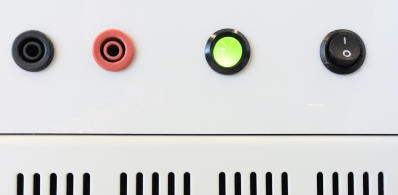
\includegraphics{zdroj2.jpg}}}
\hspace{4mm}
b)\rotatebox{0}{\scalebox{0.175}{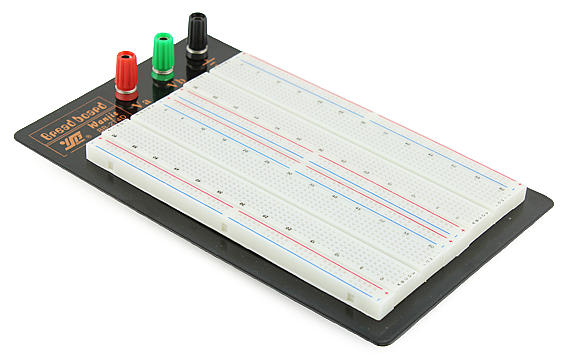
\includegraphics{pole.jpg}}}
\hspace{4mm}
c)\rotatebox{0}{\scalebox{0.125}{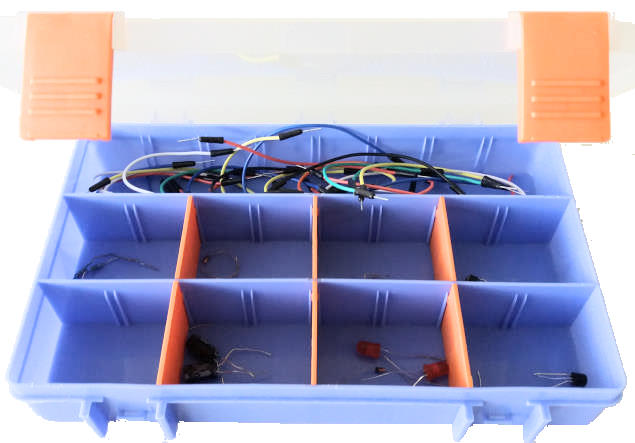
\includegraphics{box1.jpg}}}
\hspace{4mm}
d) \rotatebox{0}{
\scalebox{0.085}{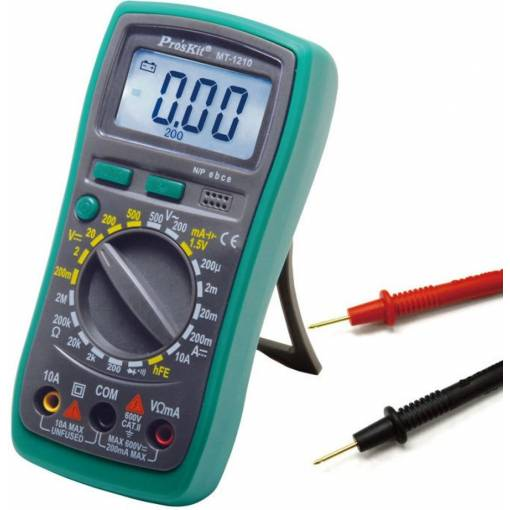
\includegraphics{multimeter/photo.jpg}}}
\hspace{4mm}
e)\rotatebox{0}{\scalebox{0.225}{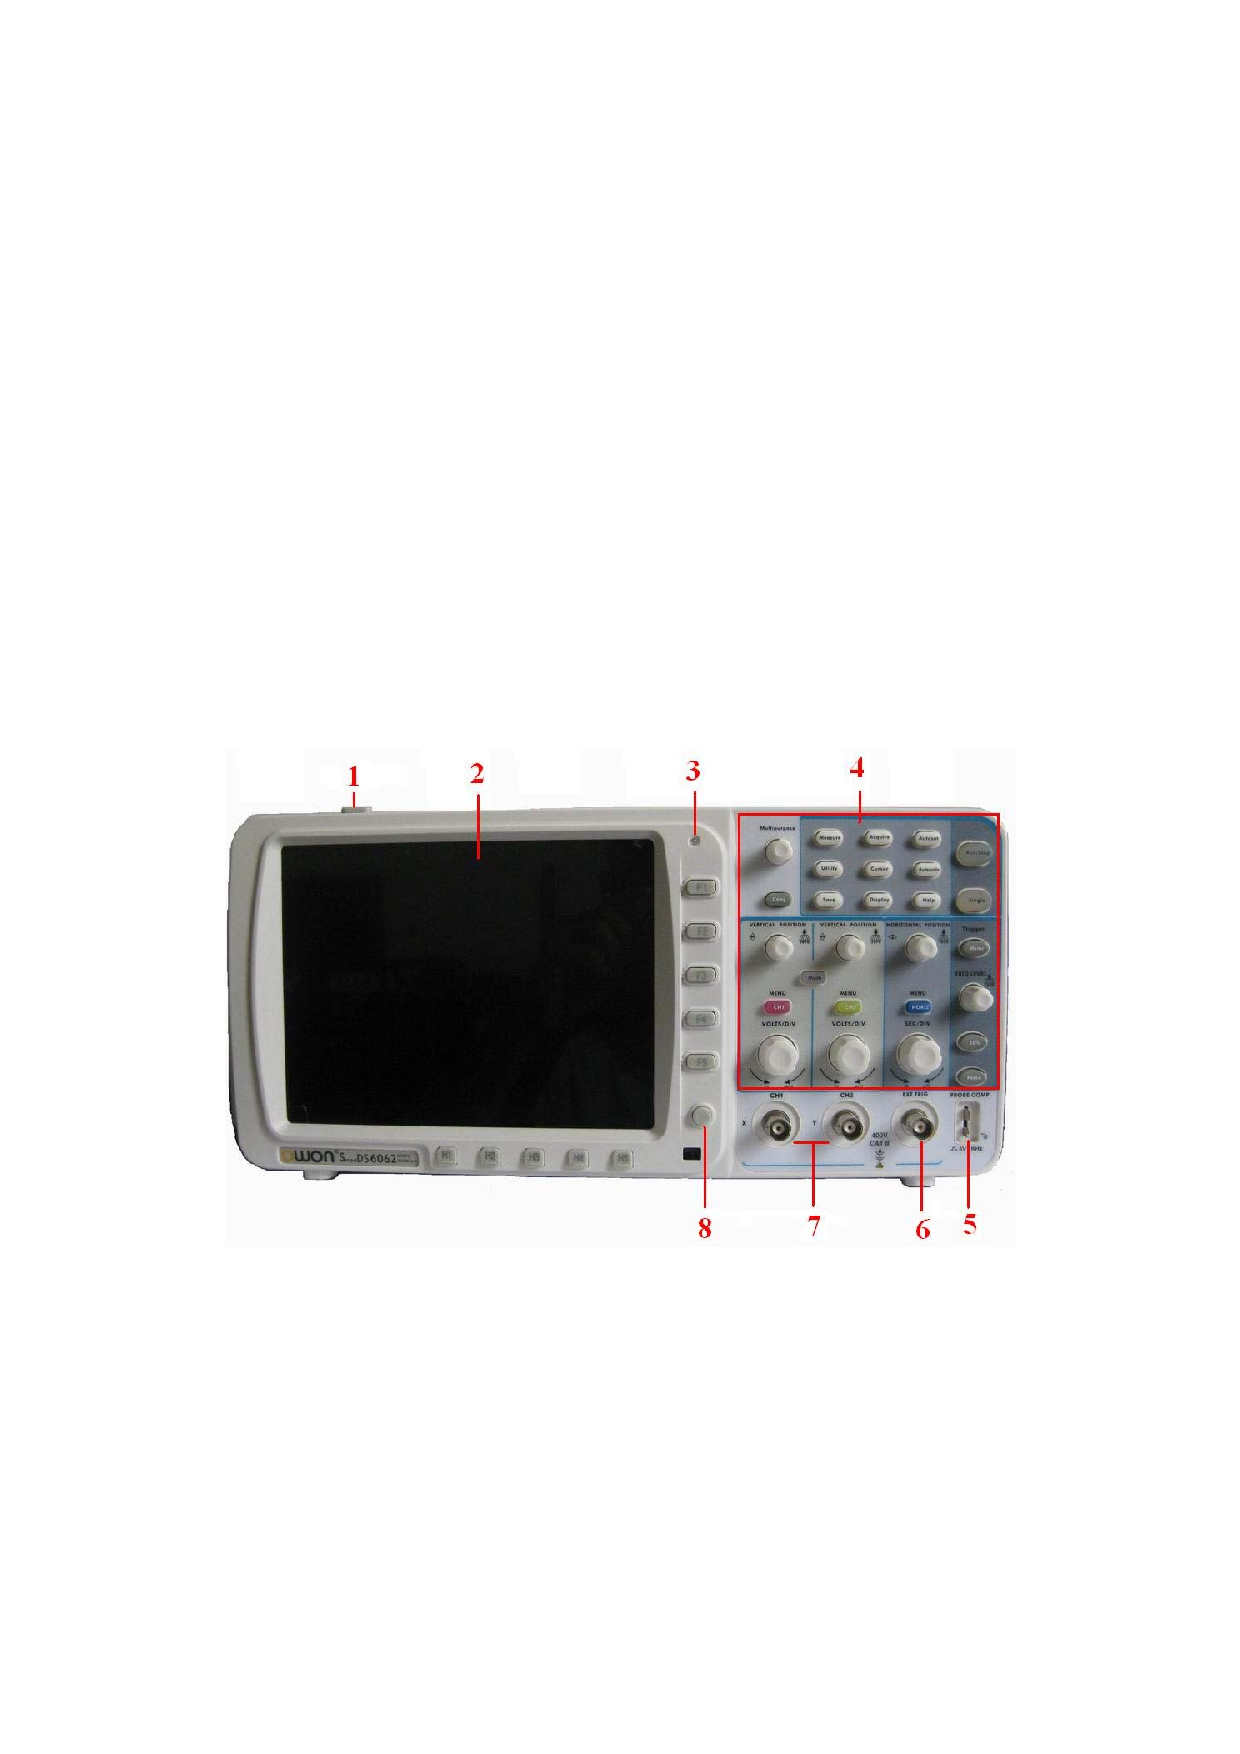
\includegraphics{oscilloscop/cut_front.pdf}}}
}
\end{center}

\vspace{-6mm}
\caption{{\bf a)} zdroj ss. napětí s omezením proudu, 
{\bf b)} nepájivé pole, 
{\bf c)} konstrukční prvky, 
{\bf d)} multimetr, 
{\bf e)} osciloskop
}
\label{sec_tools}
\end{figure}
\vspace{-5mm}

%-------------------------------------------------------------------------------
\info{Základní schéma(ta)}{aneb ,,Z čeho se bude vycházet ?''}{
~
}

\vspace{-6mm}
\begin{figure}[h!]
  \begin{center}
\scalebox{0.95}{
\parbox{2mm}{\vspace{-4mm}a)}
\hspace{4mm}
    \begin{circuitikz}
      \draw (0,2)
      to[short, o-] (1.5,2)
      to[short] (1.5,2);
      \draw[color=red] (1.5,2)
      to[ohmmeter, *-*] (1.5,0);
      \draw (1.5,0)
            to[short, -o] (0,0);
      \draw (1.5,2)
      to[short] (3,2)
      to[R, l_=$R$] (3,0) % The resistor
      to[short] (1.5,0);
    \end{circuitikz}
%
\hspace{8mm}
%
\parbox{2mm}{\vspace{-4mm}b)}
    \begin{circuitikz}
      \draw (0,0)
      to[american voltage source,invert,v<=$U$, i^=$I$] (0,2) % The voltage source
     to[short] (1.5,2);
      \draw[color=red] (1.5,2)
      to[voltmeter, *-*] (1.5,0);
      \draw (1.5,0)
      to[short] (0,0);
      \draw (1.5,2)
      to[short] (3,2)
      to[R, l_=$R$] (3,0) % The resistor
      to[short] (1.5,0);
\draw node (A) at (3.25,0) {}
node (B) at (3.25,2) {}
(A) to[open, v<=$U_R$] (B);
    \end{circuitikz}
\hspace{8mm}
\parbox{2mm}{\vspace{-4mm}c)}
    \begin{circuitikz}
      \draw (0,0)
      to[american voltage source,invert,v<=$U$, i^=$I$] (0,2) % The voltage source
      to[ammeter, color=red] (3,2)
      to[R, l_=$R$, i_=$I_R$] (3,0) % The resistor
      to[short] (0,0);
    \end{circuitikz}
}

\vspace{-2mm}
   \caption{Schémata zapojení měřicích přístrojů při měření {\bf a) odporu} R [$\Omega$] pomocí ohmmetru,
   {\bf b) napětí} U [V] pomocí voltmetru, {\bf c) proudu} I [A] pomocí ampérmetru}
   \label{sec_measurements}
  \end{center}
\vspace{-2mm}
\end{figure}

\hspace{-8mm}
\parbox{15mm}{
\dangersign[8ex]\par
}
\parbox{155mm}{
Odpor součástky a napětí na součástce odměříme tak, že měřicí přístroj zapojíme \textsc{paralelně} k součástce (tj., vedle součástky), zatímco při měření proudu zapojíme měřicí přístroj \textsc{do série} se součástkou (tj., před/za součástku).
\\
Před zahájením měření zvolené veličiny (X) vždy zkontrolujte, zda 
máte měřicí přístroj zapojen správně (viz Obr. \ref{sec_measurements})
a nastaven na měření X vč. očekávaného rozsahu hodnot;
při bližší neznalosti rozsahu X začněte nejširším rozsahem, který máte k dispozici.
}

%-------------------------------------------------------------------------------
\info{Postup samostatných činností}{aneb ,,Co dělat a na co si dát pozor ?''}{
~
}

\vspace{-8mm}
\begin{enumerate}[\bf {Experiment} 1:]

\item
\begin{enumerate}[i)]
\item 
Seznamte se s obsluhou multimetru a s Obr. \ref{sec_measurements}.
Připravte si rezistor, pomocí multimetru změřte hodnotu jeho odporu $R$ (viz Obr. \ref{sec_measurements}a) a zaznamenejte si ji\footnote{zjistěte parametry rezistoru např. pomocí \url{cz.mouser.com/technical-resources/conversion-calculators/resistor-color-code-calculator}, \url{play.google.com/store/apps/details?id=com.vivid_planet.resistor}}. 
\item Připojte rezistor ke zdroji elektrického napětí $U$. 
\item Multimetrem změřte napětí $U_R$ na rezistoru (viz Obr. \ref{sec_measurements}b) 
a proud $I_R$ procházející rezistorem (viz Obr. \ref{sec_measurements}c).

{\bf Zjistěte:}
\it Vede přiložení napětí U na rezistor R ke vzniku proudu I procházejícím rezistorem?
    Jaký vztah platí mezi U, I a R? 
\end{enumerate}

\item
\begin{enumerate}[i)]
\item Připravte si rezistor. Jeden z vývodů rezistoru spojte s pólem + napájecího zdroje (tj. s potenciálem +5 V), druhý vývod rezistoru ponechejte nezapojený. 
\item Změřte napětí $U_R$ na rezistoru.

{\bf Objasněte}
\it fyzikální princip, který je příčinou naměřené hodnoty $U_R$. 
\end{enumerate}

\item ({\it pozn.: postup proveďte odděleně pro každé ze schémat z Obr. \ref{sec_resistors}})
\vspace{-2mm}
\begin{enumerate}[i)]
\item Připravte si dva rezistory a zjistěte hodnoty jejich odporu ($R_1$, $R_2$).
\item Rezistory zapojte sériově (Obr. \ref{sec_resistors}a) 
resp. 
paralelně 
(Obr. \ref{sec_resistors}b) mezi body $A$, $B$.
\item Změřte odpor mezi body $A$ a $B$ ($R_{AB}$).
\item Mezi body $A$ a $B$ přiložte napětí $U_{AB} = 5~V$ (viz Obr. \ref{sec_resistors}).

{\bf Zjistěte:}
\it Jaký je vztah mezi $R_1$, $R_2$ a $R_{AB}$, 
	mezi $I_{R_1}$, $I_{R_2}$, $I_{AB}$ resp. 
    mezi $U_{R_1}$, $U_{R_2}$, $U_{AB}$, na čem závisí a který fyzikální zákon s ním souvisí? 
\end{enumerate}



\begin{figure}[h!]
\vspace{-4mm}
  \begin{center}
\scalebox{0.85}{
    \begin{circuitikz}
      \draw (-1,0)
      to[short, i^={$I_{AB}$}, o-] (0,0)
      to[R, l_=$R_1$, v^>=$U_{R_1}$] (3,0) % The resistor
      to[short, i^={$I_{R_1}$}] (4,0)
      to[R, l_=$R_2$, v^>=$U_{R_2}$] (7,0) % The resistor
      to[short, i^={$I_{R_2}$}, -o] (8,0)
      ;
\draw node (A) at (-1.25,0) {A};
\draw node (B) at (8.25,0) {B};
\draw node (A) at (-1,1) {}
node (B) at (8.0,1) {}
(B) to[open, v<=$U_{AB}$] (A);
    \end{circuitikz}
}
\hspace{5mm}
\scalebox{0.85}{
    \begin{circuitikz}
      \draw (0,0)
      to[short, i^={$I_{AB}$}, o-*] (1,0)
      ;
      \draw (1,1)
      to[short] (1,-1)
      ;
      \draw (1,1)
      to[short, i_=$I_{R_1}$] (2,1)
      to[R, l_=$R_1$, v^>=$U_{R_1}$] (5,1) % The resistor
      to[short, i_=$I_{R_1}$] (6,1)
      ;
      \draw (1,-1)
      to[short, i^=$I_{R_2}$] (2,-1)
      to[R, l^=$R_2$, v_>=$U_{R_2}$] (5,-1) % The resistor
      to[short, i^=$I_{R_2}$] (6,-1)
      ;
      \draw (6,1)
      to[short] (6,-1)
      ;
      \draw (6,0)
      to[short, i^={$I_{AB}$}, *-o] (7,0)
      ;
\draw node (A) at (-0.25,0) {A};
\draw node (B) at (7.25,0) {B};
\draw node (A) at (1.0,-0.25) {}
node (B) at (6.25,-0.25) {}
(B) to[open, v<={\hspace{15mm}$U_{AB}$}] (A);
    \end{circuitikz}
}

\vspace{-6mm}
{\footnotesize
a)\hspace{60mm}b)
}

\vspace{-2mm}
   \caption{Zapojení dvojice rezistorů: {\bf a) sériové}, tj. za sebou, {\bf b) paralelní}, tj. vedle sebe}
   \label{sec_resistors}
  \end{center}
\end{figure}
\vspace{-6mm}





\end{enumerate}

%-------------------------------------------------------------------------------
\info{Shrnutí, vyhodnocení a interpretace výsledků}{aneb ,,Jaká jsou zjištění ?''}{
Co byste si měli z 
této laboratoře
odnést?
Přinejmenším 
praktickou zkušenost s měřicím řetězcem (tj. s~posloupností ``měřená veličina, měřicí přístroj, výsledek měření''), chybou měření\protect\footnotemark 
~a měli byste chápat rozdíl mezi ideální a reálnou (s příslušnou tolerancí vyrobenou) součástkou.
Dále byste si měli odnést 
zjištění, že mezi $U$, $I$ a $R$ existuje závislost 
vyjádřitelná  fyzikální zákony (Ohmův z., Kirchhoffovy z.). 
}

\refstepcounter{footnote}
\footnotetext{pro více viz např. \url{https://www.amt.cz/index.php?id=CL_CHYB}}
\addtocounter{footnote}{-1}

%-------------------------------------------------------------------------------
\info{K zamyšlení/zapamatování}{aneb ,,Něco do dalšího studia a života.''}{
V této laboratoři ověřené principy/zákony mají mnohé využití. Např., s jejich pomocí můžete (teoretický pohled) elektrické obvody zjednodušit a usnadnit si tak jejich řešení, (praktický pohled) zvýšit/snížit hodnotu odporu mezi dvěma uzly, elektrického proudu obvodem či vytvořit napěťo- vý/proudový dělič s daným dělicím poměrem.
V neposlední řadě jste mohli na této laboratoři zjistit, že 
veličiny reálných součástek a 
jejich měření jsou vždy zatíženy chybou ovlivněnou mnoha faktory.
}

\end{document}
